\chapter{Advanced Algorithms}
\label{chap:advanced_algorithms}

\begin{figure}[ht]
	\hfill
	\begin{minipage}{0.5\textwidth}
		\centering
		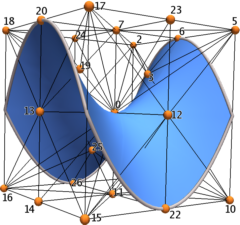
\includegraphics{VTKTextbook-168}
		\caption*{\texttt{An isocontour of a tri--quadratic Lagrange--interpolantion. Image courtesy D. Thompson and P. Pébay Sandia National Labs.}}
	\end{minipage}
\end{figure}

\firstletter{W}e return again to visualization algorithms.
This chapter describes algorithms that are either more complex to implement, or less widely used for 3D visualization applications.
We retain the classification of algorithms as either scalar, vector, tensor, or modelling algorithms.

\section{Scalar Algorithms}

As we have seen, scalar algorithms often involve mapping scalar values through a lookup table, or creating contour lines or surfaces.
In this section, we examine another contouring algorithm, dividing cubes , which generates contour surfaces using dense point clouds.
We also describe carpet plots.
Carpet plots are not true 3D visualization techniques, but are widely used to visualize many types of scalar data.
Finally, clipping is another important algorithm related to contouring, where cells are cut into pieces as a function of scalar value.

\subsection{Dividing Cubes}

Dividing cubes is a contouring algorithm similar to marching cubes \cite{Cline88}. Unlike marching cubes, dividing cubes generates point primitives as compared to triangles (3D) or lines (2D). If the number of points on the contour surface is large, the rendered appearance of the contour surface appears "solid."q To achieve this solid appearance, the density of the points must be at or greater than screen resolution. (Also, the points must be rendered using the standard lighting and shading equations used in surface rendering.)

The motivation for dividing cubes is that rendering points is much faster than rendering polygons. This varies depending upon rendering hardware/software. Special purpose hardware has been developed to render shaded points at high speed. In other systems, greater attention has been placed on polygon rendering, and the rendering speed differences are not so great. Also, certain geometric operations such as clipping and merging data are simple operations with points. Comparable operations with polygons are much more difficult to implement.

One disadvantage of creating contours with dense point clouds is that magnification of the surface (via camera zooming, for example) reveals the disconnected nature of the surface. Thus, the point set must be constructed for maximum zoom, or constructed dynamically based on the relative relationship between the camera and contour.

Although dividing cubes was originally developed for volume datasets, it is possible to adapt the algorithm to other dataset types by subdividing in parametric coordinates. Our presentation assumes that we are working with volumes.

\begin{figure}[!htb]
    \centering
    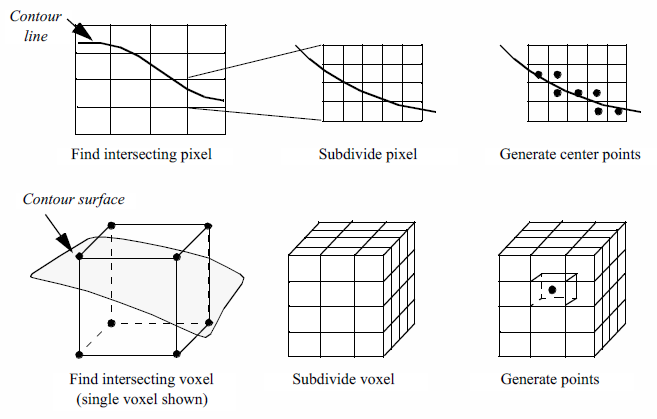
\includegraphics[width=0.98\textwidth]{Figure9-1}\\
    \caption{Overview of the dividing cubes algorithm. Voxels through which the contour passes are subdivided into subvoxels at less than screen resolution. If the contour passes through a subvoxel, a center point is generated.}\label{fig:Figure9-1}
\end{figure}

Figure \ref{fig:Figure9-1} provides an overview of the dividing cubes algorithm. Like other contouring algorithms, we first choose a contour value. We begin by visiting each voxel and select those through which the isosurface passes. (The isosurface passes through a voxel when there are scalar values both above and below the contour value.) We also compute the gradient at each voxel point for use in computing point normals.

After selecting a voxel that the isosurface passes through, the voxel is subdivided into a regular grid of $n1 \times n2 \times n3$ subvoxels. The number of divisions is controlled by the width of a voxel $w_i$ in combination with screen resolution $R$. The screen resolution is defined as the distance between adjacent pixels in world coordinates. We can express the number of divisions ni along the coordinate axes $x_i$ as $w_i$

\begin{equation}\label{eq:9.1}
n_i = \dfrac{w_i}{R}
\end{equation}
\myequations{Number of divisions along a coordinate axis.}

where the quotient is rounded up to the nearest integer. The scalar values at the subpoints are generated using the interpolation functions for a voxel (see Figure \ref{fig:Figure8-10}). Then we determine whether the contour passes through each subvoxel. If it does, we simply generate a point at the center of the subvoxel and compute its normal using the standard interpolation functions.

\begin{figure}[!htb]
    \centering
    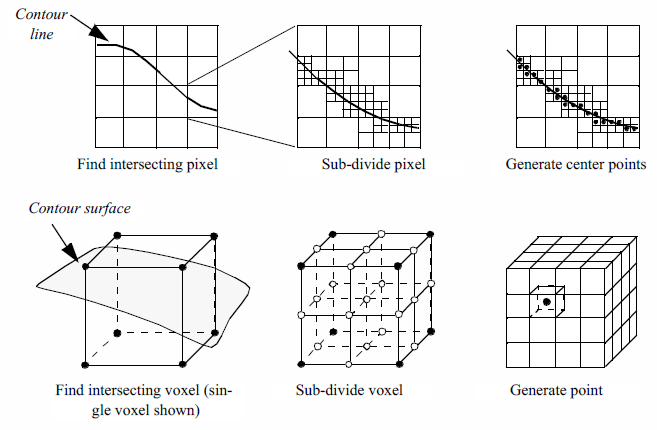
\includegraphics[width=0.98\textwidth]{Figure9-2}\\
    \caption{Recursive dividing cubes algorithm. Top half of figure shows algorithm depicted in two dimensions. Lower half depicts algorithm in three dimensions.}\label{fig:Figure9-2}
\end{figure}

An interesting variation on this algorithm is a recursive implementation as shown in Figure \ref{fig:Figure9-2}. Instead of subdividing the voxel directly (i.e., procedurally) into a regular grid we recursively divide the voxel (similar to octree decomposition). The voxel is subdivided regularly creating eight subvoxels and 19 new points (12 midedge points, 6 midface points, and 1 midvoxel point). The scalar values at the new points are interpolated from the original voxel using the trilinear interpolation functions. The process repeats for each subvoxel if the isosurface passes through it. This process continues until the size of the subvoxel is less than or equal to screen resolution. In this case, a point is generated at the center of the subvoxel. The collection of all such points composes the dividing cube's isosurface.

The advantage of the recursive implementation is that the subdivision process terminates prematurely in those regions of the voxel where the contour cannot pass. On the other hand, the recursive subdivision requires that the voxel subdivision occurs in powers of two. This can generate far more points than the procedural implementation.

\begin{figure}[!htb]
    \centering
    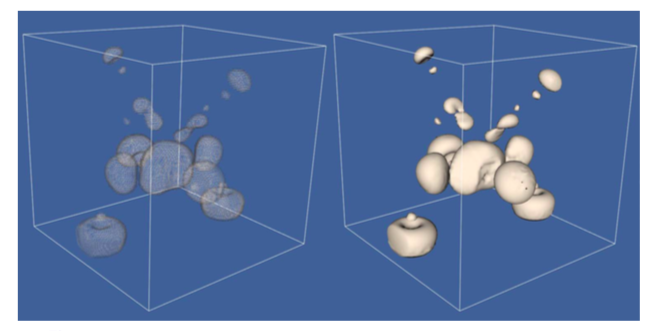
\includegraphics[width=0.98\textwidth]{Figure9-3}\\
    \caption{Examples of dividing cubes isosurface. The left image consists of 50,078 points, and the right image consists of 2,506,989 points.}\label{fig:Figure9-3}
\end{figure}

Figure \ref{fig:Figure9-3} shows two examples of dividing cubes isosurfaces. The contour surface on the left consists of 50,078 points. Because the points are not generated at display resolution, it is possible to see through the contour surface. The second contour surface on the right is composed of 2,506,989 points. The points are generated at display resolution, and as a result the contour surface appears solid.

As Figure \ref{fig:Figure9-1} and Figure \ref{fig:Figure9-2} show, the points generated by dividing cubes do not lie exactly on the contour surface. We can determine the maximum error by examining the size of the terminal subvoxels. Assume that a terminal subvoxel is a cube, and that the length of the side of the cube is given by $l$. Then the maximum error is half the length of the cube diagonal, or $l \sqrt{3} / 2$.

\subsection{Carpet Plots}

A common data form is a 2D image dataset with associated scalar data. Carpet plots can visualize data in this form. A carpet plot is created by warping a 2D surface in the direction of the surface normal (or possibly some user-defined direction). The amount of warping is controlled by the scalar value, possibly in combination with a scale factor. Carpet plots are similar to the vector displacement plots (see ``Displacement Plots'' on page \pageref{subsec:displacement_plots})

Although carpet plots are typically applied to image data, they can be used to visualize datasets composed of 2D structured grids or 2D unstructured grids. In their basic form carpet plots can be used to visualize only three variables: two surface position coordinates and a scalar value. However, it is common to introduce another variable by using color mapping on the surface.

\begin{figure}[!htb]
    \centering
    \begin{subfigure}{0.48\linewidth}
        \centering
        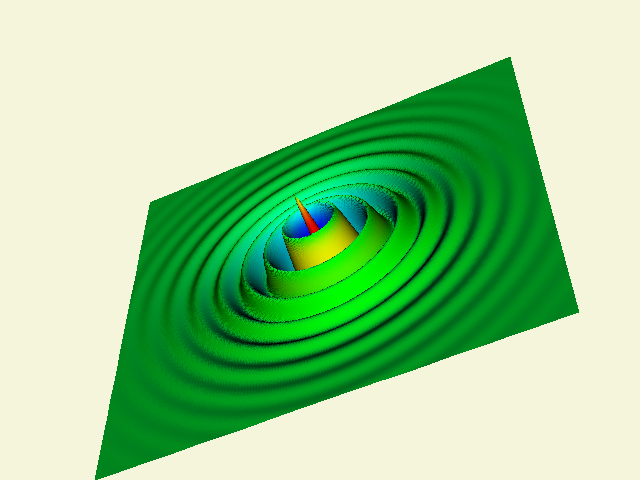
\includegraphics[width=.96\linewidth]{Figure9-4a}
        \caption{Exponential cosine function.(\href{https://lorensen.github.io/VTKExamples/site/Cxx/VisualizationAlgorithms/ExponentialCosine/}{ExponentialCosine.cxx} or \href{https://lorensen.github.io/VTKExamples/site/Python/VisualizationAlgorithms/ExponentialCosine/}{ExponentialCosine.py})}\label{fig:Figure9-4a}
    \end{subfigure}
    \hfill
    \begin{subfigure}{0.48\linewidth}
        \centering
        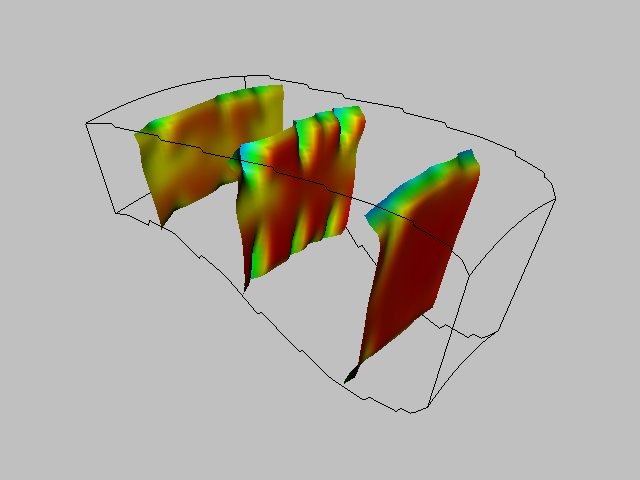
\includegraphics[width=.96\linewidth]{Figure9-4b}
        \caption{Flow energy.(\href{https://lorensen.github.io/VTKExamples/site/Cxx/VisualizationAlgorithms/WarpCombustor/}{WarpCombustor.cxx} or \href{https://lorensen.github.io/VTKExamples/site/Python/VisualizationAlgorithms/WarpCombustor/}{WarpCombustor.py})}\label{fig:Figure9-4b}
    \end{subfigure}%
    \caption{Carpet plot. (a) Visualization of an exponential cosine function. Function values are indicated by surface displacement. Colors indicate derivative values. Carpet plot of combustor flow energy in a structured grid. Colors and plane displacement represent energy values.}
    \label{fig:Figure9-4}
\end{figure}

Figure \ref{fig:Figure9-4} illustrates application of carpet plots. Figure \ref{fig:Figure9-4}(a) shows the exponential cosine function centered at the origin with points located at radius $r$

\begin{equation}\label{eq:9.2}
F(r) = e^{-r}\cos(10\, r)
\end{equation}
\myequations{Exponential cosine function.}

The function values are used to warp the surface while the function derivatives are used to color it. Figure \ref{fig:Figure9-4}(b) shows a carpet plot that visualizes flow energy in a structured grid. Both displacement and color are used to show the energy values. Although this figure is similar to Figure \ref{fig:Figure6-14}(b) there are some important differences. Figure \ref{fig:Figure6-14}(b) displays vector data whereas Figure \ref{fig:Figure9-4}(b) displays scalar data. Figure \ref{fig:Figure9-4}(b) deforms the surface in the direction of surface normal (or possibly a user-defined direction). The vector data (i.e., vector orientation) controls the direction of deformation in Figure \ref{fig:Figure6-14}(b).

\subsection{Clipping With Scalar Fields}
\label{subsec:clipping_with_scalar_fields}

\begin{figure}[!htb]
    \centering
    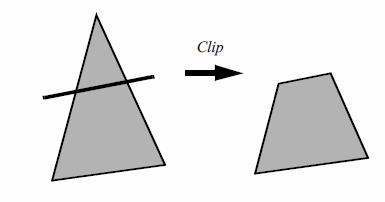
\includegraphics[width=0.98\textwidth]{Figure9-5}\\
    \caption{Clipping a triangle produces a polygon. The dark line represents an infinite plane.}\label{fig:Figure9-5}
\end{figure}


Clipping is a common graphics operation that limits the extent of a polygon so that it does not lie outside the view frustrum (see on page ``Cameras'' on page \pageref{sec:cameras}). Figure \ref{fig:Figure9-5} shows a triangle before and after clipping with an infinite plane. The clip operation transforms a polygon into a polygon. Clipping can also be a powerful modeling tool. Clipping part of a structure can reveal internal details of the surface or other parts contained within the surface. Objects can be split into pieces and the pieces can be individually moved and controlled.

\begin{figure}[!htb]
    \centering
    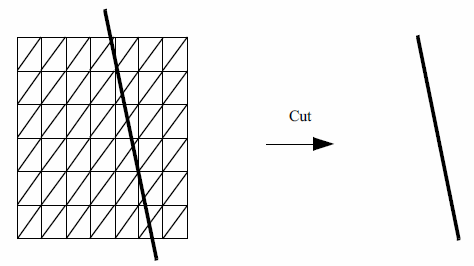
\includegraphics[width=0.98\textwidth]{Figure9-6}\\
    \caption{Cutting polygons produces lines (cutPlane.tcl).}\label{fig:Figure9-6}
\end{figure}

\begin{figure}[!htb]
    \centering
    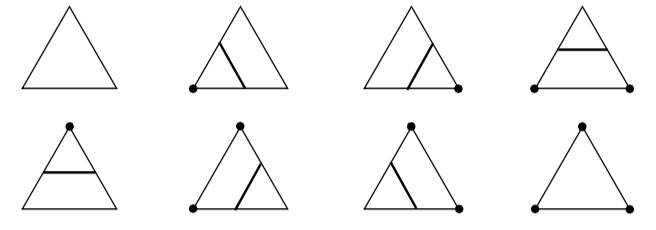
\includegraphics[width=0.98\textwidth]{Figure9-7}\\
    \caption{The eight cases for cutting (contouring) a triangle. Black dots show triangle vertices that are ``inside'' the scalar cutting region. Solid lines show the output of the cutting operation.}\label{fig:Figure9-7}
\end{figure}

We can do clipping with arbitrary implicit functions using a variation of the ``marching'' primitives discussed in ``Contouring''on page \ref{subsec:contouring}. We illustrate the technique for triangles.

Recall that marching triangles transforms triangles into lines that approximate a scalar value called the isovalue. This is accomplished using the inside/outside relationship that each vertex has with respect to some scalar value. For our purposes here, we use a scalar value that represents the signed distance of the triangle vertex to a plane. This infinite plane, described by an implicit function of the form $F(x, y, z) = n_{xx} + n_{yy} + n_{zz} - d = 0$, partitions space into two infinite half spaces. All points with negative scalar values lie on one side of the plane and all with positive values lie on the other side. Figure \ref{fig:Figure9-6} shows a finite plane represented by a grid of triangles. The thick line shows the infinite plane defined by $F(x,y,z) = x + y + z - c = 0$. The cut algorithm described in ``Cutting'' on page \pageref{subsec:cutting} creates a set of lines using the contour operations specific to each cell primitive. In this example, the triangle's contour operator extracts lines that lie on the intersection of the infinite plane and the triangles that comprise the finite plane. The contour operation for a triangle uses the eight cases shown in Figure \ref{fig:Figure9-7} to contour or ``cut'' each triangle appropriately.

\begin{figure}[!htb]
    \centering
    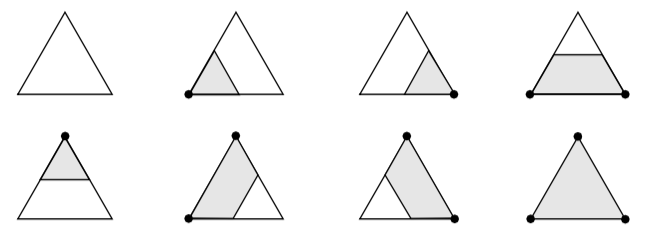
\includegraphics[width=0.98\textwidth]{Figure9-8}\\
    \caption{The eight cases for clipping a triangle. Black dots show triangle vertices that are "inside" the scalar clipping region. Shaded regions show the output of the clip operation.}\label{fig:Figure9-8}
\end{figure}

\begin{figure}[!htb]
    \centering
    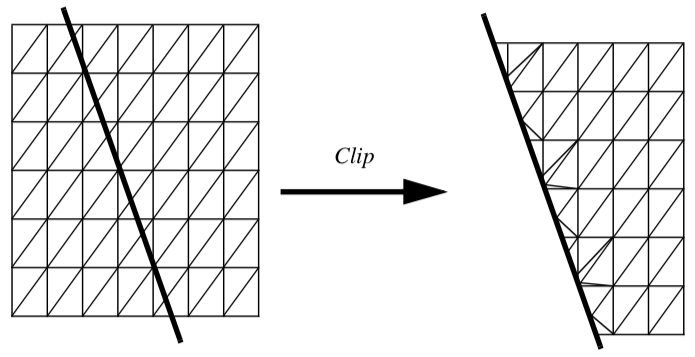
\includegraphics[width=0.98\textwidth]{Figure9-9}\\
    \caption{A plane of triangles clipped with a plane function (clipPlane.tcl).}\label{fig:Figure9-9}
\end{figure}

Clipping transforms polygons into polygons. We do clipping with a modified case table for the triangle that outputs polygons shown in Figure \ref{fig:Figure9-8}. In VTK, each polygonal data cell has a different case table to define the clip operation. Applying the clip algorithm to the polygonal data in Figure \ref{fig:Figure9-9} using the same scalar field generated with a plane equation produces a new set of triangles.

Formulating clipping using scalar fields permits more sophisticated operations. Clipping can use scalar data that is computed or scalar data that is part of a polygonal dataset's point attributes.

\begin{figure}[!htb]
    \centering
    \begin{subfigure}{0.41\linewidth}
        \centering
        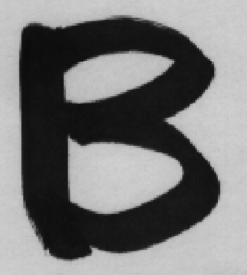
\includegraphics[width=.96\linewidth]{Figure9-10a}
        \caption*{}\label{fig:Figure9-10a}
    \end{subfigure}
    \hfill
    \begin{subfigure}{0.16\linewidth}
        \centering
        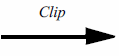
\includegraphics[width=.96\linewidth]{Figure9-10b}
        \caption*{}\label{fig:Figure9-10b}
    \end{subfigure}%
    \hfill
    \begin{subfigure}{0.41\linewidth}
        \centering
        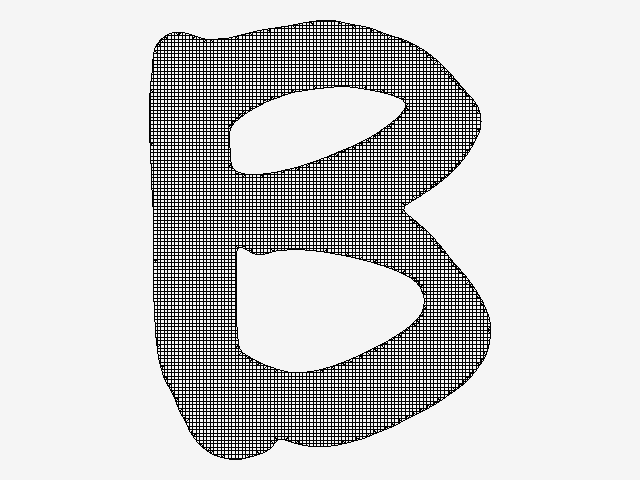
\includegraphics[width=.96\linewidth]{Figure9-10c}
        \caption*{(\href{https://lorensen.github.io/VTKExamples/site/Cxx/VisualizationAlgorithms/CreateBFont/}{CreateBFont.cxx} or \href{https://lorensen.github.io/VTKExamples/site/Python/VisualizationAlgorithms/CreateBFont/}{CreateBFont.py})}\label{fig:Figure9-10c}
    \end{subfigure}%
    \caption{Carpet plot. (a) Visualization of an exponential cosine function. Function values are indicated by surface displacement. Colors indicate derivative values. Carpet plot of combustor flow energy in a structured grid. Colors and plane displacement represent energy values.}
    \label{fig:Figure9-10}
\end{figure}

Figure \ref{fig:Figure9-10} shows a scanned image that is first converted to a quadrilateral mesh with vertex scalar values set to the scanned image intensity. Clipping this quadrilateral mesh with a value equal to 1/2 the maximum intensity of the scanned image produces a polygonal model show in Figure \ref{fig:Figure9-10}.

\section{Vector Algorithms}

In Chapter 6: \nameref{chap:fundamental_algorithms} we showed how to create simple vector glyphs and how to integrate particles through a vector field to create streamlines. In this section we extend these concepts to create streamribbons and streampolygons. In addition, we introduce the concept of vector field topology, and show how to characterize a vector field using topological constructs.

\subsection{Streamribbons and Streamsurfaces}

Streamlines depict particle paths in a vector field. By coloring these lines, or creating local glyphs (such as dashed lines or oriented cones), we can represent additional scalar and temporal information. However, these techniques can convey only elementary information about the vector field. Local information (e.g., flow rotation or derivatives) and global information (e.g., structure of a field such as vortex tubes) is not represented. Streamribbons and streamsurfaces are two techniques used to represent local and global information.

A natural extension of the streamline technique widens the line to create a ribbon. The ribbon can be constructed by generating two adjacent streamlines and then bridging the lines with a polygonal mesh. This technique works well as long as the streamlines remain relatively close to one another. If separation occurs, so that the streamlines diverge, the resulting ribbon will not accurately represent the flow, because we expect the surface of the ribbon to be everywhere tangent to the vector field (i.e., definition of streamline). The ruled surface connecting two widely separated streamlines does not generally satisfy this requirement.

The streamribbon provides information about important flow parameters: the vector vorticity and flow divergence. \emph{Vorticity} $\Omega$ is the measure of rotation of the vector field, expressed as a vector quantity: a direction (axis of rotation) and magnitude (amount of rotation). \emph{Streamwise vorticity} $\Omega$ is the projection of $\overrightarrow{\omega}$ along the instantaneous velocity vector, $\overrightarrow{v}$. Said another way, streamwise vorticity is the rotation of the vector field around the streamline defined as follows.

\begin{equation}\label{eq:9.3}
\Omega = \frac{\overrightarrow{v\ } \cdot \overrightarrow{\omega\ }}{\vert \overrightarrow{v\ } \vert \vert \overrightarrow{\omega\ } \vert}
\end{equation}
\myequations{Streamwise vorticity.}

The amount of twisting of the streamribbon approximates the streamwise vorticity. Flow divergence is a measure of the "spread" of the flow. The changing width of the streamribbon is proportional to the cross-flow divergence of the flow.

A streamsurface is a collection of an infinite number of streamlines passing through a \emph{base curve}. The base curve, or \emph{rake}, defines the starting points for the streamlines. If the base curve is closed (e.g., a circle) the surface is closed and a streamtube results. Thus, streamribbons are specialized types of streamsurfaces with a narrow width compared to length.

Compared to vector icons or streamlines, streamsurfaces provide additional information about the structure of the vector field. Any point on the streamsurface is tangent to the velocity vector. Consequently, taking an example from fluid flow, no fluid can pass through the surface. Streamtubes are then representations of constant mass flux. Streamsurfaces show vector field structure better than streamlines or vector glyphs because they do not require visual interpolation across icons.

Streamsurfaces can be computed by generating a set of streamlines from a user-specified rake. A polygonal mesh is then constructed by connecting adjacent streamlines. One difficulty with this approach is that local vector field divergence can cause streamlines to separate. Separation can introduce large errors into the surface, or possibly cause self-intersection, which is not physically possible.

Another approach to computing streamsurfaces has been taken by Hultquist \cite{Hultquist92}. The streamsurface is a collection of streamribbons connected along their edges. In this approach, the computation of the streamlines and tiling of the streamsurface is carried out concurrently. This allows streamlines to be added or removed as the flow separates or converges. The tiling can also be controlled to prevent the generation of long, skinny triangles. The surface may also be ``torn'', i.e., ribbons separated, if the divergence of the flow becomes too high.

\subsection{Stream Polygon}

he techniques described so far provide approximate measures of vector field quantities such as streamwise vorticity and divergence. However, vector fields contain more information than these techniques can convey. As a result, other techniques have been devised to visualize this information. One such technique is the stream polygon \cite{Schroeder91}, which serves as the basis for a number of advanced vector and tensor visualization methods. The stream polygon is used to visualize local properties of strain, displacement, and rotation. We begin by describing the effects of a vector field on the local state of strain.

Nonuniform vector fields give rise to local deformation in the region where they occur. If the vector field is displacement in a physical medium such as a fluid or a solid, the deformation consists of local strain (i.e., local distortion) and rigid body motion. To mathematically describe the deformation, we examine a 3D vector $\overrightarrow{v\ } = (u, v, w)$ at a specified point $x = (x, y, z)$. Using a first order Taylor's series expansion about $\overrightarrow{x\ }$, we can express the local deformation $e_ij$ as

\begin{equation}\label{eq:9.4}
e_{ij} = \epsilon_{ij} + \omega_{ij}
\end{equation}
\myequations{Local deformation.}

where $\epsilon_{ij}$ is the local strain and $\omega_{ij}$ is the local rotation. Note that these variables are expressed as $3 \times 3$ tensors. (Compare this equation to that given in Figure \ref{fig:Figure6-20}. Note that this equation and the following Equation \ref{eq:9.5} differ in their off-diagonal terms by a factor of $1/2$. This is because Figure \ref{fig:Figure6-20} expresses engineering shear strain which is used in the study of elasticity. Equation \ref{eq:9.5} expresses a tensor quantity and is mathematically consistent.)

The local strain is expressed as a combination of the partial derivatives at $\overrightarrow{x\ }$ as follows.

\begin{equation}\label{eq:9.5}
\mathbf{\epsilon} = \left(
\begin{array}{c c c}
  \dfrac{\partial u}{\partial x} &
  \dfrac{1}{2}\left(\dfrac{\partial u}{\partial y} + \dfrac{\partial v}{\partial x}\right) &
  \dfrac{1}{2}\left(\dfrac{\partial u}{\partial z} + \dfrac{\partial w}{\partial x}\right) \\ \\
  \dfrac{1}{2}\left(\dfrac{\partial u}{\partial y} + \dfrac{\partial v}{\partial x}\right) &
  \dfrac{\partial v}{\partial y} &
  \dfrac{1}{2}\left(\dfrac{\partial v}{\partial z} + \dfrac{\partial w}{\partial y}\right) \\ \\
  \dfrac{1}{2}\left(\dfrac{\partial u}{\partial z} + \dfrac{\partial w}{\partial x}\right) &
  \dfrac{1}{2}\left(\dfrac{\partial v}{\partial z} + \dfrac{\partial w}{\partial y}\right) &
  \dfrac{\partial w}{\partial z}
\end{array}\right)
\end{equation}
\myequations{Local strain.}

The terms on the diagonal of $\epsilon_{ij}$ are the normal components of strain. The off-diagonal terms are the shear strain. The local rigid--body rotation is given by

\begin{equation}\label{eq:9.6}
\mathbf{\omega} = \left(
\begin{array}{c c c}
  0 &
  \dfrac{1}{2}\left(\dfrac{\partial u}{\partial y} - \dfrac{\partial v}{\partial x}\right) &
  \dfrac{1}{2}\left(\dfrac{\partial u}{\partial z} - \dfrac{\partial w}{\partial x}\right) \\ \\
  \dfrac{1}{2}\left(\dfrac{\partial v}{\partial x} - \dfrac{\partial u}{\partial y}\right) &
  0 &
  \dfrac{1}{2}\left(\dfrac{\partial v}{\partial z} - \dfrac{\partial w}{\partial y}\right) \\ \\
  \dfrac{1}{2}\left(\dfrac{\partial w}{\partial x} - \dfrac{\partial u}{\partial z}\right) &
  \dfrac{1}{2}\left(\dfrac{\partial w}{\partial y} - \dfrac{\partial v}{\partial z}\right) &
  0
\end{array}\right)
\end{equation}
\myequations{Local rigid--body rotation.}

Equation \ref{eq:9.6} can also be represented using tensor notation as

\begin{equation}\label{eq:9.7}
\omega_{ij} = -\dfrac{1}{2}\sum_{k} \epsilon_{ijk}\, \omega_{k}
\end{equation}
\myequations{Local deformation.}

where $\overrightarrow{\omega\ }$ is the vorticity vector referred to in the previous section. The vorticity, or local rigid body rotation is then

\begin{equation}\label{eq:9.8}
\overrightarrow{\omega\ } = \left(
\begin{array}{c}
\dfrac{\partial w}{\partial y} - \dfrac{\partial v}{\partial z} \\ \\
\dfrac{\partial u}{\partial z} - \dfrac{\partial w}{\partial x} \\ \\
\dfrac{\partial v}{\partial x} - \dfrac{\partial u}{\partial y}
\end{array}
\right)
\end{equation}
\myequations{Vorticity vector.}

\begin{figure}[htb]
	\begin{subfigure}[h]{0.48\linewidth}
		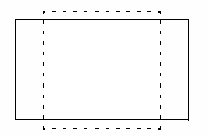
\includegraphics[width=0.96\linewidth]{Figure9-11a}
		\captionsetup{justification=centering}
		\caption{Normal strain}
		\label{fig:Figure9-11a}
	\end{subfigure}
	\hfill
	\begin{subfigure}[h]{0.48\linewidth}
		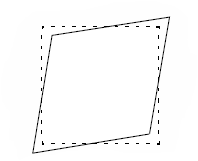
\includegraphics[width=0.96\linewidth]{Figure9-11b}
		\captionsetup{justification=centering}
		\caption{Shear strain}
		\label{fig:Figure9-11b}
	\end{subfigure}
	\hfill
	\begin{subfigure}[h]{0.48\linewidth}
		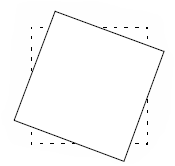
\includegraphics[width=0.96\linewidth]{Figure9-11c}
		\captionsetup{justification=centering}
		\caption{Rotation}
		\label{fig:Figure9-11c}
	\end{subfigure}
	\hfill
		\begin{subfigure}[h]{0.48\linewidth}
		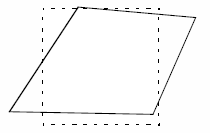
\includegraphics[width=0.96\linewidth]{Figure9-11d}
		\captionsetup{justification=centering}
		\caption{Total deformation}
		\label{fig:Figure9-11d}
	\end{subfigure}
	\caption{Components of local deformation due to vector field. Dotted line shows initially undeformed object.}\label{fig:Figure9-11}
\end{figure}

For the reader unfamiliar with tensor notation, this presentation is certainly less than complete. However, the matrices in Equation \ref{eq:9.5} and Equation \ref{eq:9.6} directly translate into visual form, which will help clarify the concepts presented here. Referring to Figure \ref{fig:Figure9-11}, the normal strain, shear strain, and rigid body motion create distinct deformation modes. These modes combine to produce the total deformation. Modes of normal strain cause compression or extension in the direction perpendicular to a surface, while shear strains cause angular distortions. These strains combined with rigid body rotation around an axis yield the total strain at a point.

\begin{figure}[htb]
	\begin{subfigure}[h]{0.48\linewidth}
		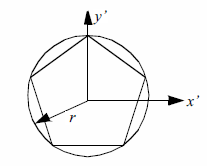
\includegraphics[width=0.96\linewidth]{Figure9-12a}
		\captionsetup{justification=centering}
		\caption{Planar view}
		\label{fig:Figure9-12a}
	\end{subfigure}
	\hfill
	\begin{subfigure}[h]{0.48\linewidth}
		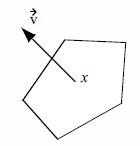
\includegraphics[width=0.96\linewidth]{Figure9-12b}
		\captionsetup{justification=centering}
		\caption{Normal to vector}
		\label{fig:Figure9-12b}
	\end{subfigure}
	\hfill
	\begin{subfigure}[h]{0.48\linewidth}
		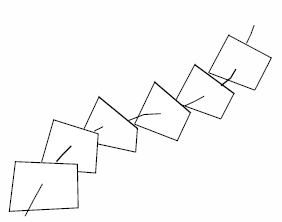
\includegraphics[width=0.96\linewidth]{Figure9-12c}
		\captionsetup{justification=centering}
		\caption{Placed along streamline}
		\label{fig:Figure9-12c}
	\end{subfigure}
	\hfill
		\begin{subfigure}[h]{0.48\linewidth}
		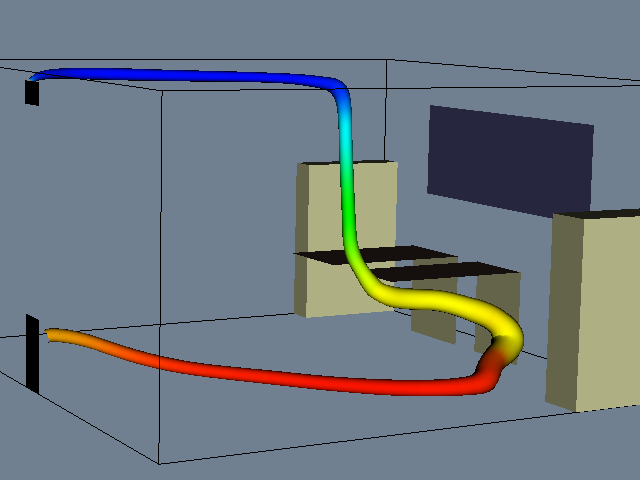
\includegraphics[width=0.96\linewidth]{Figure9-12d}
		\captionsetup{justification=centering}
		\caption{Stream tube(\href{https://lorensen.github.io/VTKExamples/site/Cxx/VisualizationAlgorithms/OfficeTube/}{OfficeTube.cxx} or \href{https://lorensen.github.io/VTKExamples/site/Python/VisualizationAlgorithms/OfficeTube/}{OfficeTube.py})}
		\label{fig:Figure9-12d}
	\end{subfigure}
	\caption{The stream polygon. (a) Planar view. (b) Aligned with vector. (c) Aligned along streamline. (d) Sweeping polygon to form tube.}\label{fig:Figure9-12}
\end{figure}

The essence of the stream polygon technique is to show these modes of deformation. A regular \emph{n}--sided polygon (Figure \ref{fig:Figure9-12}) is placed into a vector field at a specified point and then deformed according to the local strain. The components of strain may be shown separately or in combination. The orientation of the normal of the polygon is arbitrary. However, it is convenient to align the normal with the local vector. Then the rigid body rotation about the vector is the streamwise vorticity, and the effects of normal and shear strain are in the plane perpendicular to a streamline passing through the point.

The stream polygon offers other interesting possibilities. The stream polygon may be swept along a trajectory, typically a streamline, to generate tubes. The radius of the tube $r$ can be modified according to some scalar function. One application is to visualize fluid flow. In incompressible flow with no shear, the radius of the tube can vary according to the scalar function vector magnitude. Then the equation

\begin{equation}\label{eq:9.9}
r(\overrightarrow{v\ }) = r_\text{max} \sqrt{\dfrac{\vert\overrightarrow{v}_\text{min}\vert}{\vert\overrightarrow{v\ }\vert}}
\end{equation}
\myequations{Area of constant mass flow.}

represents an area of constant mass flow. As a result, the tube will thicken as the flow slows and narrow as the velocity increases. Each of the \emph{n} sides of the tube can be colored with a different scalar function, although for visual clarity, at most, one or two functions should be used.

The streamtubes generated by the streampolygon and the streamtubes we described in the previous section are not the same. The streampolygon does not necessarily lie along a streamline. If it does, the streampolygon represents information at a point, while the streamtube is an approximation constructed from multiple streamlines. Also, the radial variation in the tubes constructed from streampolygon sweeps do not necessarily relate to mass flow since the radius in a streampolygon can be tied to an arbitrary scalar variable.

\subsection{Vector Field Topology}

Vector fields have a complex structure characterized by special features called critical points \cite{Globus91} \cite{Helman91}. Critical points are locations in the vector field where the local vector magnitude goes to zero and the vector direction becomes undefined. At these points the vector field either converges or diverges, and/or local circulation around the point occurs.

Critical points lie in dataset cells where the u, v, and w components of the vector field each pass through zero. These points are located using an iterative search procedure such as the bi-section technique. Each iteration evaluates the cell interpolation function until the zero vector is found. Once a critical point is found, its local behavior is determined from the matrix of partial derivatives.

This is because at the critical point the velocity is zero, and the vector field can be approximated by a first-order expansion of partial derivatives \cite{Helman91}

\begin{equation}\label{eq:9.10}
\begin{array}{lll}
u &\simeq& \dfrac{\partial u}{\partial x}\text{d}x
         + \dfrac{\partial u}{\partial y}\text{d}y
         + \dfrac{\partial u}{\partial z}\text{d}z \\ \\
v &\simeq& \dfrac{\partial v}{\partial x}\text{d}x
         + \dfrac{\partial v}{\partial y}\text{d}y
         + \dfrac{\partial v}{\partial z}\text{d}z \\ \\
w &\simeq& \dfrac{\partial w}{\partial x}\text{d}x
         + \dfrac{\partial w}{\partial y}\text{d}y
         + \dfrac{\partial w}{\partial z}\text{d}z
\end{array}
\end{equation}
\myequations{Approximation of a vector field.}

The matrix of partial derivatives $J$ can be written in vector notation as $\partial u \partial v \partial w$

\begin{equation}\label{eq:9.11}
\overrightarrow{u\ } = \mathbf{J}\cdot\text{d}\overrightarrow{x },\quad \text{where} \quad \mathbf{J} = \left(
\begin{array}{c c c}
\dfrac{\partial u}{\partial x} & \dfrac{\partial u}{\partial y} & \dfrac{\partial u}{\partial z} \\ \\
\dfrac{\partial v}{\partial x} & \dfrac{\partial v}{\partial y} & \dfrac{\partial v}{\partial z} \\ \\
\dfrac{\partial w}{\partial x} & \dfrac{\partial w}{\partial y} & \dfrac{\partial w}{\partial z}
\end{array}
\right)
\end{equation}
\myequations{The Jacobian.}

and is referred to as the Jacobian. The behavior of the vector field in the vicinity of a critical point is characterized by the eigenvalues of $J$. The eigenvalues consist of an imaginary and real component. The imaginary component describes the rotation of the vector field around the critical point, while the real part describes the relative attraction or repulsion of the vector field to the critical point. In two dimensions the critical points are as shown in Figure\ref{fig:Figure9-13}.

\begin{figure}[htb]
	\begin{subfigure}[h]{0.32\linewidth}
		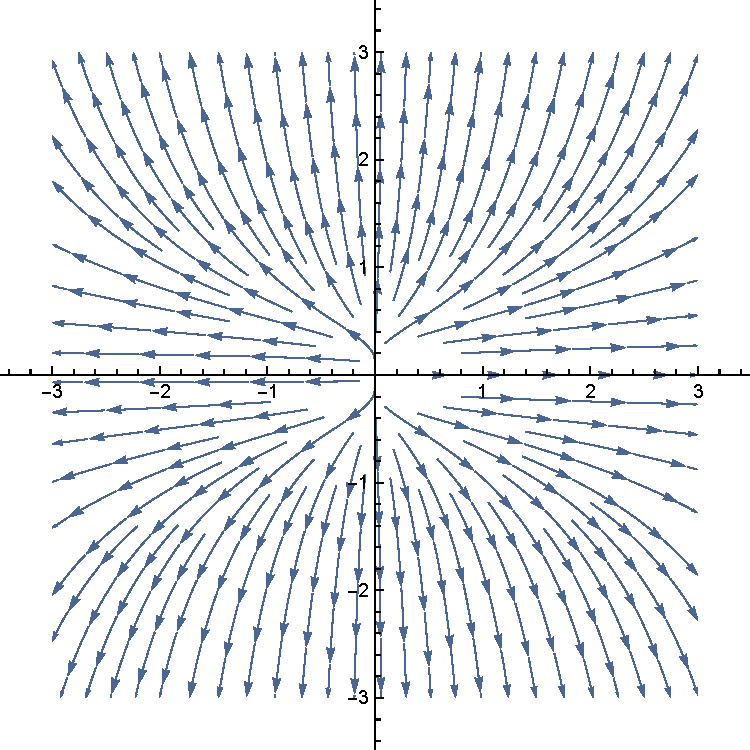
\includegraphics[width=0.86\linewidth]{Figure9-13a}
		\captionsetup{justification=centering}
		\caption*{Repelling Node\\$R_1, R_2 > 0$\\$I_1, I_2 = 0$}
		\label{fig:Figure9-13a}
	\end{subfigure}
	\hfill
	\begin{subfigure}[h]{0.32\linewidth}
		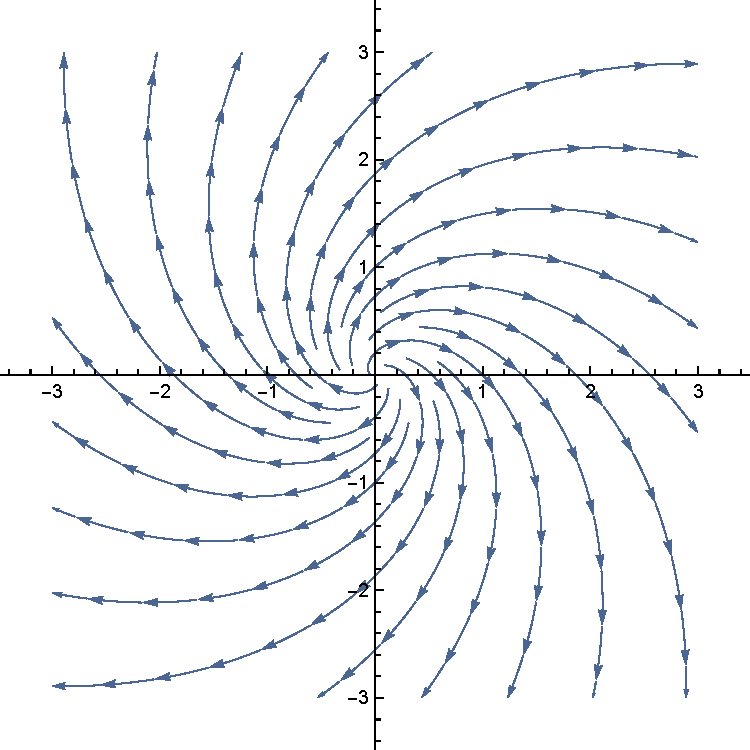
\includegraphics[width=0.86\linewidth]{Figure9-13b}
		\captionsetup{justification=centering}
		\caption*{Repelling Focus\\$R_1, R_2 > 0$\\$I_1, I_2 \neq 0$}
		\label{fig:Figure9-13b}
	\end{subfigure}
	\hfill
	\begin{subfigure}[h]{0.32\linewidth}
		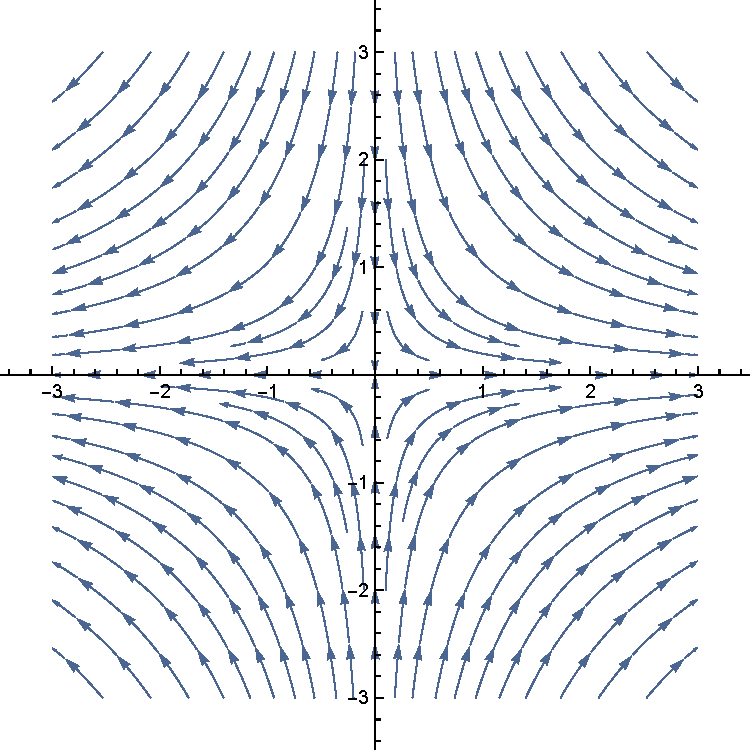
\includegraphics[width=0.86\linewidth]{Figure9-13c}
		\captionsetup{justification=centering}
		\caption*{Saddle Point\\$R_1 \times R_2 < 0$\\$I_1, I_2 = 0$}
		\label{fig:Figure9-13c}
	\end{subfigure}
	\hfill
		\begin{subfigure}[h]{0.32\linewidth}
		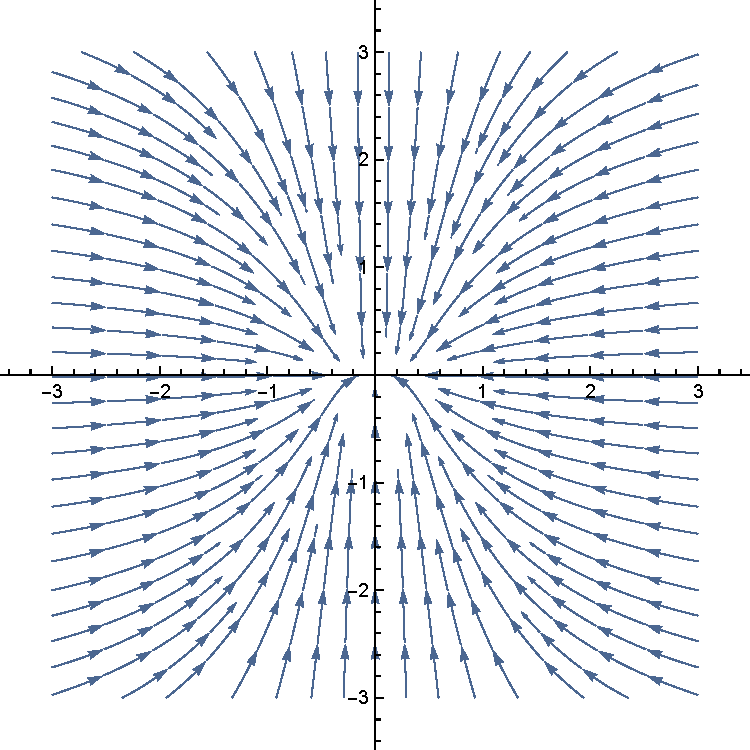
\includegraphics[width=0.86\linewidth]{Figure9-13d}
		\captionsetup{justification=centering}
		\caption*{Attracting Node\\$R_1, R_2 < 0$\\$I_1, I_2 = 0$}
		\label{fig:Figure9-13d}
	\end{subfigure}
	\hfill
	\begin{subfigure}[h]{0.32\linewidth}
		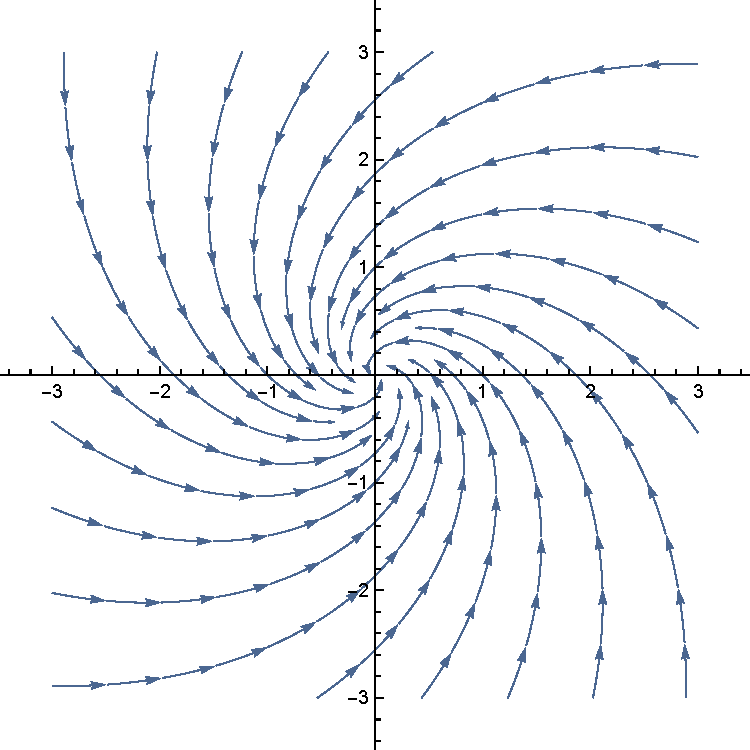
\includegraphics[width=0.86\linewidth]{Figure9-13e}
		\captionsetup{justification=centering}
		\caption*{Attracting Focus\\$R_1, R_2 < 0$\\$I_1, I_2 \neq 0$}
		\label{fig:Figure9-13e}
	\end{subfigure}
	\hfill
	\begin{subfigure}[h]{0.32\linewidth}
		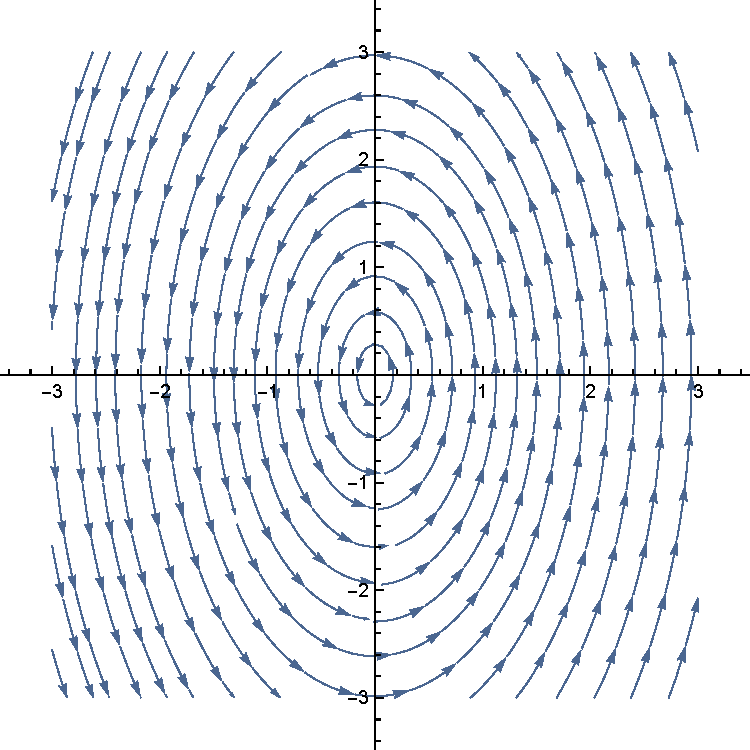
\includegraphics[width=0.86\linewidth]{Figure9-13f}
		\captionsetup{justification=centering}
		\caption*{Center\\$R_1, R_2 = 0$\\$I_1, I_2 \neq 0$}
		\label{fig:Figure9-13f}
	\end{subfigure}
	\caption{Critical points in two dimensions. The real part of the eigenvalues ($R_1$, $R_2$) of the matrix of first derivatives control the attraction or repulsion of the vector field. The imaginary part of the eigenvalues ($I_1$, $I_2$) controls the rotation.}\label{fig:Figure9-13}
\end{figure}

A number of visualization techniques have been developed to construct vector field topology from an analysis of critical points. These techniques provide a global understanding of the field, including points of attachment and detachment and field vortices. Using a fluid flow analogy, points of attachment and detachment occur on the surface of an object where the tangential component of the vector field goes to zero, and the flow is perpendicular to the surface. Thus, streamlines will begin or end at these points. There is no common definition for a vortex, but generally speaking, vortices are regions of relatively concentrated vorticity (e.g., flow rotation). The study of vortices is important because they represent areas of energy loss, or can have significant impact on downstream flow conditions (e.g., trailing vortices behind large aircraft).

One useful visualization technique creates vector field skeletons that divide the vector field into separate regions. Within each region, the vector field is topologically equivalent to uniform flow. These skeletons are created by locating critical points, and then connecting the critical points with streamlines. In 3D vector field analysis this technique can be applied to the surface of objects to locate lines of flow separation and attachment and other important flow features. Also, in general 3D flow, the regions of uniform flow are separated by surfaces, and creation of 3D flow skeletons is a current research topic.

Vortex visualization is another area of current research. One technique computes the \emph{helicitydensity}

\begin{equation}\label{eq:9.12}
H_d = \overrightarrow{v\ } \cdot \overrightarrow{w\ } = \vert \overrightarrow{v\ } \vert \vert \overrightarrow{w\ } \vert \cos(\phi)
\end{equation}
\myequations{Scalar function of the vector dot product. }

This is a scalar function of the vector dot product between the vorticity and the local vector. Large positive values of $H_d$ result in right-handed vortices, while large negative values indicate lefthanded vortices. Helicity-density can be conveniently shown using isosurfaces, which gives an indication for the location and structure of a vortex.

\section{Tensor Algorithms}

In Chapter 6: \nameref{chap:fundamental_algorithms} we saw that $3 \times 3$ real symmetric tensors can be characterized by the eigenvalues and eigenvectors of the tensor. Recall that we can express the eigenvectors of the system as

\begin{equation}\label{eq:9.13}
\overrightarrow{v\ } = \sum_i \lambda_i \overrightarrow{e\ }_i
\end{equation}
\myequations{Eigenvalues of a system. }

where $\overrightarrow{e\ }_i$ is a unit vector in the direction of the eigenvalue, and $\lambda_i$ are the eigenvalues. Thus, we can decompose a  $3 \times 3$ real symmetric tensor field into three vector fields, each field defined by one of the three eigenvectors described in Equation \ref{eq:9.13}. We call these vector fields \emph{eigenfields}, since they are derived from the eigenvectors of the tensor field.

Decomposition of the tensor field in this fashion provides additional insight into visualizing $3 \times 3$ real symmetric tensors. We can directly use the vector field visualization techniques presented previously or use variations of them. One such technique is a novel extension of the streampolygon technique, the method of \emph{hyperstreamlines}.

\subsection{Hyperstreamlines}

\begin{figure}[htb]
	\begin{subfigure}[h]{0.48\linewidth}
		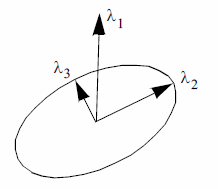
\includegraphics[width=0.66\linewidth]{Figure9-14a}
		\captionsetup{justification=centering}
		\caption{Ellipse definition}
		\label{fig:Figure9-14a}
	\end{subfigure}
	\hfill
	\begin{subfigure}[h]{0.48\linewidth}
		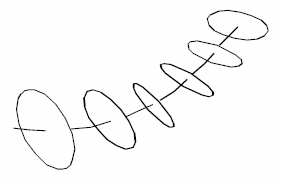
\includegraphics[width=0.96\linewidth]{Figure9-14b}
		\captionsetup{justification=centering}
		\caption{Ellipse swept to create tube}
		\label{fig:Figure9-14b}
	\end{subfigure}
	\caption{Creation of hyperstreamlines. An ellipse is swept along a streamline of the eigenfield. Major/minor axes of the ellipse are controlled by the other two eigenvectors.}\label{fig:Figure9-14}
\end{figure}

Hyperstreamlines are constructed by creating a streamline through one of the three eigenfields, and then sweeping a geometric primitive along the streamline \cite{Delmarcelle93}. Typically, an ellipse is used as the geometric primitive, where the remaining two eigenvectors define the major and minor axes of the ellipse (Figure \ref{fig:Figure9-14}). Sweeping the ellipse along the eigenfield streamline results in a tubular shape. Another useful generating geometric primitive is a cross. The length and orientation of the arms of the cross are controlled by two of the eigenvectors. Sweeping the cross results in a helical shape since the eigenvectors (and therefore cross arms) will rotate in some tensor fields.

\begin{figure}[!htb]
	\floatbox[{\capbeside\thisfloatsetup{capbesideposition={right,center},capbesidewidth=0.4\textwidth}}]{figure}[\FBwidth]
	{\caption{The four hyperstreamlines shown are integrated along the minor principle stress axis. A plane (colored with a different lookup table) is also shown.(\href{https://lorensen.github.io/VTKExamples/site/Cxx/VisualizationAlgorithms/HyperStreamline/}{HyperStreamline.cxx} or \href{https://lorensen.github.io/VTKExamples/site/Python/VisualizationAlgorithms/HyperStreamline/}{HyperStreamline.py}}\label{fig:Figure9-15}}
	{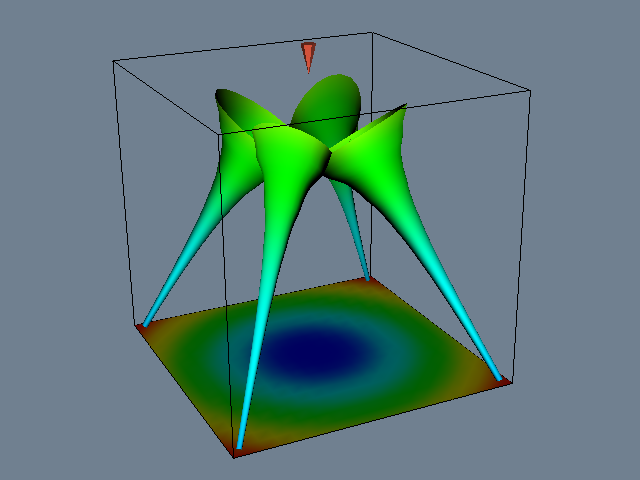
\includegraphics[width=0.6\textwidth]{Figure9-15}}
\end{figure}


Figure \ref{fig:Figure9-15} shows an example of hyperstreamlines. The data is from a point load applied to a semi-infinite domain. Compare this figure to Figure \ref{fig:Figure6-22} that used tensor ellipsoids to visualize the same data. Notice that there is less clutter and more information available from the hyperstreamline visualization.



\section{Modelling Algorithms}

\subsection{Visualizing Geometry}

One of the most common applications of visualization is to view geometry. We may have a geometric representation of a part or complex assembly (perhaps designed on a CAD system) and want to view the part or assembly before it is manufactured. While viewing geometry is better addressed in text on computer graphics, often there is dataset structure we wish to view in the same way. For example, we may want to see data mapped on a particular portion of the dataset, or view the structure of the dataset itself (e.g., view a finite element mesh).

Three-dimensional datasets have a surface and interior. Typically we want to visualize the surface of the dataset or perhaps a portion of the interior. (Note: volume rendering is a different matter - see ``Volume Rendering'' on page \pageref{sec:volume_rendering}). To visualize the dataset we must extract a portion of the dataset topology/geometry (and associated data) as some form of surface primitives such as polygons. If the surface of the dataset is opaque, we may also wish to eliminate occluded interior detail.

We have already seen how structured datasets, such as image data or structured grids, have a natural $i-j-k$ coordinate system that allow extraction of points, lines, and planes from the interior of the dataset (see ``Structured Coordinate System'' on page \pageref{subsec:structured_coordinate_system})). For example, to extract the fifth $-$iplane from a structured grid of dimensions $(i_m, j_m, k_m)$, we specify the data extents using $(4, 4, 0, (j_m - 1), 0, (k_m 1))$ (assuming zero-offset addressing).

\begin{figure}[htb]
	\begin{subfigure}[h]{0.48\linewidth}
		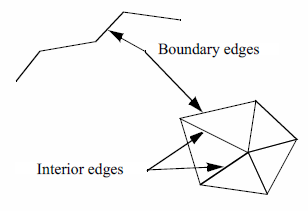
\includegraphics[width=0.96\linewidth]{Figure9-16a}
		\captionsetup{justification=centering}
		\caption*{}
		\label{fig:Figure9-16a}
	\end{subfigure}
	\hfill
	\begin{subfigure}[h]{0.48\linewidth}
		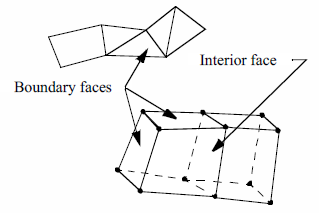
\includegraphics[width=0.96\linewidth]{Figure9-16b}
		\captionsetup{justification=centering}
		\caption*{}
		\label{fig:Figure9-16b}
	\end{subfigure}
	\caption{Boundary edges and faces.}\label{fig:Figure9-16}
\end{figure}

More generally, we can extract boundary edges and faces from a dataset. A boundary edge is an 1D cell type (e.g., line or polyline), or the edge of a 2D cell used by only that single cell. Similarly, a boundary face is a 2D cell type (e.g., polygon, triangle strip) or the face of a 3D cell used by only that single cell (Figure \ref{fig:Figure9-16}). We can obtain this information using the topological operators of the previous chapter. Cells of dimensions two or less are extracted as is, while boundary edges and faces are determined by counting the number of cell neighbors for a particular topological boundary (i.e., edge or face neighbors). If there are no neighbors, the edge or face is a boundary edge or face, and is extracted.

Using these techniques we can view the structure of our dataset. However, there are also situations where we want more control in the selection of the data. We call this \emph{data extraction}.

\subsection{Data Extraction}

Often we want to extract portions of data from a dataset. This may be because we want to reduce the size of the data, or because we are interested in visualizing only a portion of it.

Reducing dataset size is an important practical capability, because visualization data size can be huge. By reducing data size, reductions in computation and memory requirements can be realized. This results in better interactive response.

We also may need to reduce data size in order to visualize the important features of a large dataset. This can be used to reduce image clutter and improve the effectiveness of the visualization. Smaller data size also enables the visualization user to navigate through and inspect data more quickly relative to larger datasets. Next we describe two techniques to extract data. One is based on geometry extraction, and the other is based on data thresholding, or thresholding.

\subsubsection{Geometry Extraction}

Geometry extraction selects data based on geometric or topological characteristics. A common extraction technique selects a set of points and cells that lie within a specified range of ids. A typical example is selecting all cells having ids between 0-100, or all cells using point ids 250-500. Finite element analysts use this method frequently to isolate the visualization to just a few key regions.

\begin{figure}[htb]
	\begin{subfigure}[h]{0.48\linewidth}
		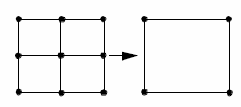
\includegraphics[width=0.96\linewidth]{Figure9-17a}
		\captionsetup{justification=centering}
		\caption{Subsampling structured data}
		\label{fig:Figure9-17a}
	\end{subfigure}
	\hfill
	\begin{subfigure}[h]{0.48\linewidth}
		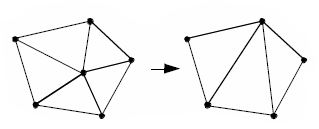
\includegraphics[width=0.96\linewidth]{Figure9-17b}
		\captionsetup{justification=centering}
		\caption{Subsampling unstructured data}
		\label{fig:Figure9-17b}
	\end{subfigure}
	\caption{Subsampling data. (a) Structured data can be subsampled by choosing every nth point. (b) Subsampling unstructured data requires local retriangulation.}\label{fig:Figure9-17}
\end{figure}

Another useful technique called spatial extraction, selects dataset structure and associated data attributes lying within a specified region in space. For example, a point and radius can be used to select (or deselect) data within an enclosing sphere. Implicit functions are particularly useful tools for describing these regions. Points that evaluate negative are inside the region, while points outside the region evaluate positive; thus, cells whose points are all positive are outside the region, and cells whose points are all negative are inside the region.

\emph{Subsampling} (Figure \ref{fig:Figure9-17}) is a method that reduces data size by selecting a subset of the original data. The subset is specified by choosing a parameter n, specifying that every nth data point is to be extracted. For example, in structured datasets such as image data and structured grids, selecting every nth point produces the results shown in igure \ref{fig:Figure9-17}(a).

Subsampling modifies the topology of a dataset. When points or cells are not selected, this leaves a topological ``hole''. Dataset topology must be modified to fill the hole. In structured data, this is simply a uniform selection across the structured $i-j-k$ coordinates. In unstructured data (Figure \ref{fig:Figure9-17}(b)), the hole must be filled in by using triangulation or other complex tessellation schemes. Subsampling is not typically performed on unstructured data because of its inherent complexity.

A related technique is \emph{data masking}. In data masking we select every $n^{th}$ cell that at a minimum leaves one or more topological ``holes'' in the dataset. Masking also may change the topology of the dataset, since partial selections of cells from structured datasets can only be represented using unstructured grids. Masking is typically used to improve interactive performance or to quickly process portions of data.

\subsubsection{Thresholding}

Thresholding extracts portions of a dataset data based on attribute values. For example, we may select all cells having a point with scalar value between (0,1) or all points having a velocity magnitude greater than 1.0.

Scalar thresholding is easily implemented. The threshold is either a single value that scalar values are greater than or less than, or a range of values. Cells or points whose associated scalar values satisfy the threshold criteria can be extracted. Other dataset attribute types such as vectors, normals, or tensors can be extracted in similar fashion by converting the type to a single scalar value. For example, vectors can be extracted using vector magnitude, and tensors using matrix determinate.

A problem with both geometry extraction and thresholding is that the approaches presented thus far extract ``atomic'' pieces of data, that is, a complete cell. Sometimes the cell may lie across the boundary of the threshold. In this case the cell must be clipped (see ``Clipping With Scalar Fields'' on page \pageref{subsec:clipping_with_scalar_fields} and only a portion of the cell is extracted.

\subsection{Probing}

Probing obtains dataset attributes by sampling one dataset (the input) with a set of points (the probe) as shown in Figure \ref{fig:Figure9-18}(a). Probing is also called ``resampling''. Examples include probing an input dataset with a sequence of points along a line, on a plane, or in a volume. The result of the probing is a new dataset (the output) with the topological and geometric structure of the probe dataset, and point attributes interpolated from the input dataset. Once the probing operation is completed, the output dataset can be visualized with any of the appropriate techniques described in this text.

\begin{figure}[htb]
	\begin{subfigure}[h]{0.48\linewidth}
		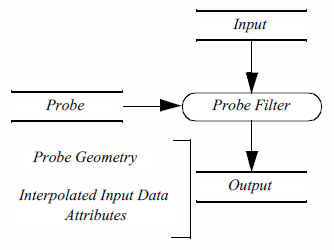
\includegraphics[width=0.96\linewidth]{Figure9-18a}
		\captionsetup{justification=centering}
		\caption{Probing process}
		\label{fig:Figure9-18a}
	\end{subfigure}
	\hfill
	\begin{subfigure}[h]{0.48\linewidth}
		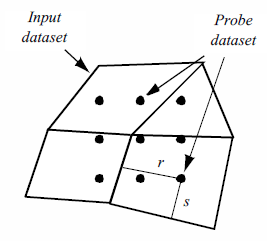
\includegraphics[width=0.96\linewidth]{Figure9-18b}
		\captionsetup{justification=centering}
		\caption{Probe interpolation}
		\label{fig:Figure9-18b}
	\end{subfigure}
	\caption{Probing. The geometry of one dataset \textit{(Probe)} is used to extract dataset attributes from anther dataset \textit{(Input)}.}\label{fig:Figure9-18}
\end{figure}

Figure \ref{fig:Figure9-18}(b) illustrates the details of the probing process. For every point in the probe dataset, the location in the input dataset (i.e., cell, subcell, and parametric coordinates) and interpolation weights are determined. Then the data values from the cell are interpolated to the probe point. Probe points that are outside the input dataset are assigned a nil (or appropriate) value. This process repeats for all points in the probe dataset.

Probing can be used to reduce data or to view data in a particular fashion.

\begin{itemize}

\item Data is reduced when the probe operation is limited to a subregion of the input dataset, or the number of probe points is less than the number of input points.

\item Data can be viewed in a particular fashion by sampling on specially selected datasets. Using a probe dataset consisting of a line enables x-y plotting along a line, or using a plane allows surface color mapping or line contouring.

\end{itemize}

Probing must be used carefully or errors may be introduced. Under-sampling data in a region can miss important high-frequency information or localized data variations. Oversampling data, while not creating error, can give false confidence in the accuracy of the data. Thus the sampling frequency should have a similar density as the input dataset, or if higher density, the visualization should be carefully annotated as to the original data frequency.

One important application of probing converts irregular or unstructured data to structured form using a volume of appropriate resolution as a probe to sample the unstructured data. This is useful if we use volume rendering or other volume visualization techniques to view our data.

\begin{figure}[!htb]
	\floatbox[{\capbeside\thisfloatsetup{capbesideposition={right,center},capbesidewidth=0.4\textwidth}}]{figure}[\FBwidth]
	{\caption{Probing data in a combustor.  Probes are regular arrays of $50^2$ points that are then passed through a contouring filter.(\href{https://lorensen.github.io/VTKExamples/site/Cxx/VisualizationAlgorithms/ProbeCombustor/}{ProbeCombustor.cxx} or \href{https://lorensen.github.io/VTKExamples/site/Python/VisualizationAlgorithms/ProbeCombustor/}{ProbeCombustor.py})}\label{fig:Figure9-19}}
	{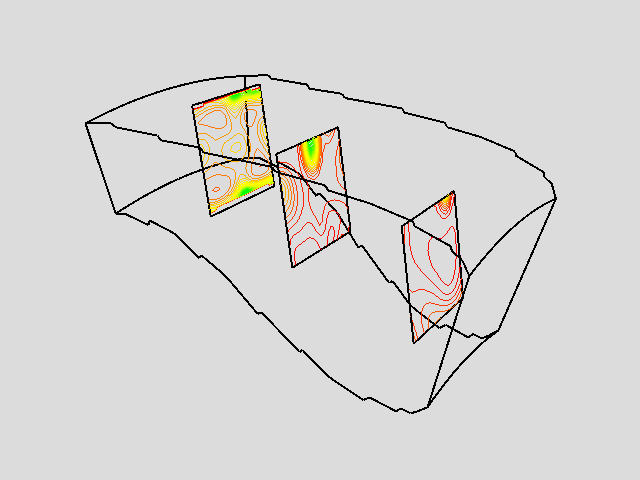
\includegraphics[width=0.6\textwidth]{Figure9-19}}
\end{figure}

Figure \ref{fig:Figure9-19} shows an example of three probes. The probes sample flow density in a structured grid. The output of the probes is passed through a contour filter to generate contour lines. As this figure illustrates, we can be selective with the location and extent of the probe, allowing us to focus on important regions in the data.

\subsection{Triangle Strip Generation}

Triangle strips are compact representations of triangle polygons as described in ``Triangle Strip'' on page \pageref{subsec:linear_cells.triangle_strip}. Many rendering libraries include triangle strips as graphics primitives because they are a high-performance alternative to general polygon rendering.

Visualization and graphics data is often represented with triangles. Marching cubes, for example, generates thousands and potentially millions of triangles to represent an isosurface. To achieve greater performance in our visualizations, we can convert triangle polygons into triangle strips. Or, if data is represented using polygons, we can first triangulate the polygons and then create triangle strips.

\begin{figure}[htb]
	\begin{subfigure}[h]{0.48\linewidth}
		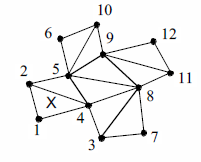
\includegraphics[width=0.96\linewidth]{Figure9-20a}
		\captionsetup{justification=centering}
		\caption*{Select first triangle}
		\label{fig:Figure9-20a}
	\end{subfigure}
	\hfill
	\begin{subfigure}[h]{0.48\linewidth}
		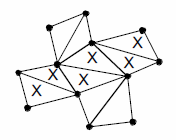
\includegraphics[width=0.96\linewidth]{Figure9-20b}
		\captionsetup{justification=centering}
		\caption*{Extend strip}
		\label{fig:Figure9-20b}
	\end{subfigure}
	\begin{subfigure}[h]{0.48\linewidth}
		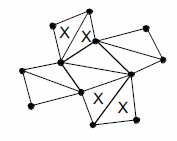
\includegraphics[width=0.96\linewidth]{Figure9-20c}
		\captionsetup{justification=centering}
		\caption*{Create additional strips}
		\label{fig:Figure9-20c}
	\end{subfigure}
	\hfill
	\begin{subfigure}[h]{0.48\linewidth}
    \centering
        \begin{minipage}[b]{.4\textwidth}
        \centering
        Representation:\\
        (1,2,4,5,8,9,11,12)\\
        (6,5,10,9)\\
        (4,3,8,7)
        \end{minipage}
		\captionsetup{justification=centering}
		\caption*{}
	\end{subfigure}
	\caption{Creating triangle strips.}\label{fig:Figure9-20}
\end{figure}


A simple method to generate triangle strips uses greedy gathering of triangles into a strip (Figure \ref{fig:Figure9-20}). The method proceeds as follows. An ``unmarked'' triangle is found to initialize the strip --- unmarked triangles are triangles that have not yet been gathered into a triangle strip. Starting with the initial triangle, the strip may grow in one of three directions, corresponding to the three edges of the triangle. We choose to grow the strip in the direction of the first unmarked neighbor triangle we encounter. If there are no unmarked neighbors the triangle strip is complete; otherwise, the strip is extended by adding triangles to the list that satisfy triangle strip topology. The strip is grown until no unmarked neighbor can be found. Additional strips are then created using the same procedure until every triangle is marked.

The length of the triangle strips varies greatly depending on the structure of the triangle mesh.

\begin{figure}[!htb]
	\centering
	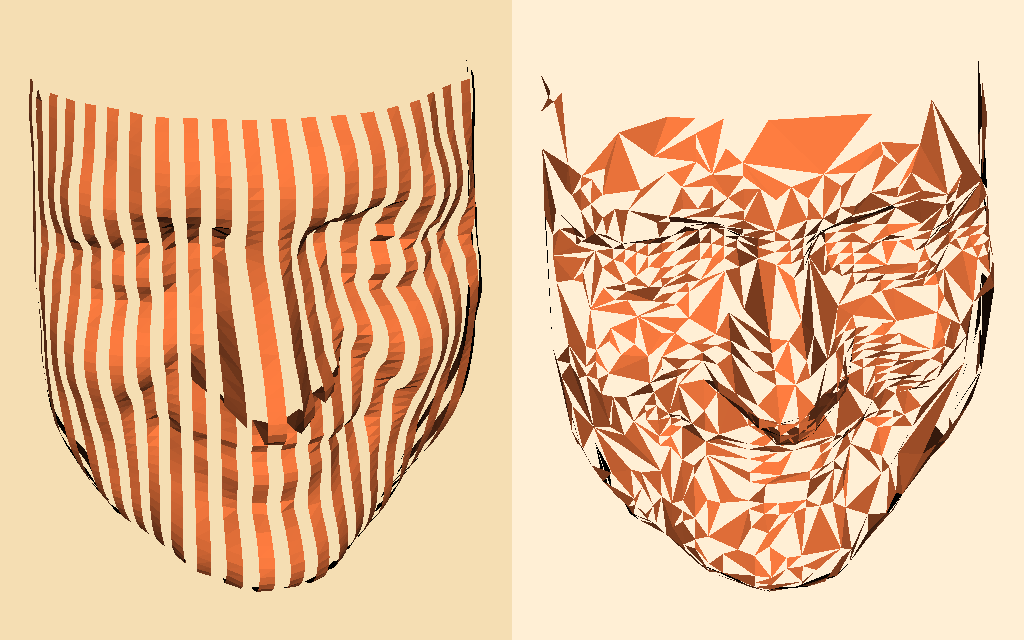
\includegraphics[width=0.98\textwidth]{Figure9-21}
	\caption{Triangle strip examples. Left, structured triangle mesh consisting of 134 strips each of 390 triangles. Right, Unstructured triangle mesh consisting of 2227 strips of average length 3.94, longest strip 101 triangles. Images are generated by displaying every other triangle strip.(\href{https://lorensen.github.io/VTKExamples/site/Cxx/Rendering/StripFran/}{StripFran.cxx} or \href{https://lorensen.github.io/VTKExamples/site/Python/Rendering/StripFran/}{StripFran.py})}
	\label{fig:Figure9-21}
\end{figure}


Figure \ref{fig:Figure9-21}(left) shows triangle strips each of 390 triangles in length from a dataset that was originally structured. Such a case is an exception: unstructured triangle meshes typically average about 5-6 triangles per strip (Figure \ref{fig:Figure9-21}(right)). Even so, the memory savings are impressive. A triangle strip of length 6 requires 8 points to represent, while 8 triangles require 24 points, for a memory savings of 66.7 percent. Rendering speed may be greatly affected, too, depending upon the capabilities of the rendering system.

\subsection{Connectivity}

\begin{figure}[htb]
	\begin{subfigure}[h]{0.32\linewidth}
		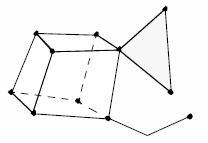
\includegraphics[width=0.96\linewidth]{Figure9-22a}
		\captionsetup{justification=centering}
		\caption*{Point connected}
		\label{fig:Figure9-22a}
	\end{subfigure}
	\hfill
	\begin{subfigure}[h]{0.32\linewidth}
		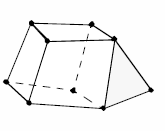
\includegraphics[width=0.96\linewidth]{Figure9-22b}
		\captionsetup{justification=centering}
		\caption*{Edge connected}
		\label{fig:Figure9-22b}
	\end{subfigure}
	\begin{subfigure}[h]{0.32\linewidth}
		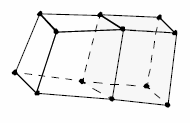
\includegraphics[width=0.96\linewidth]{Figure9-22c}
		\captionsetup{justification=centering}
		\caption*{Face connected}
		\label{fig:Figure9-22c}
	\end{subfigure}
	\caption{Connected cells.}\label{fig:Figure9-22}
\end{figure}

Intercell connectivity is a topological property of datasets. Cells are topologically connected when they share boundary features such as points, edges, or faces (Figure \ref{fig:Figure9-22}). Connectivity is useful in a number of modeling applications, particularly when we want to separate out ``parts'' of a dataset.


\begin{figure}[!htb]
	\centering
	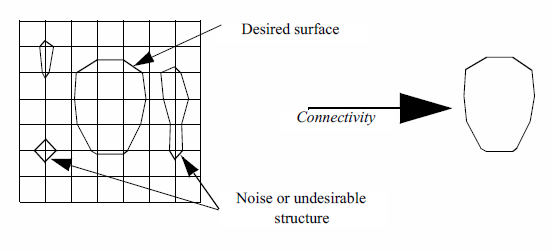
\includegraphics[width=0.98\textwidth]{Figure9-23}
	\caption{Extracting portion of isosurface of interest using connectivity.}
	\label{fig:Figure9-23}
\end{figure}

One application of connectivity extracts a meaningful portion of an isosurface. If the isosurface is generated from measured data such as an MRI or CT scan, it likely contains ``noise'' or unimportant anatomical structure. Using connectivity algorithms, we can separate out the part of the isosurface that we desire, either by eliminating noise or undesirable anatomical structure. Figure \ref{fig:Figure9-23} is an example where a 2D surface of interest (e.g., an isocontour) is extracted from a noisy signal.

Connectivity algorithms can be implemented using a recursive visit method. We begin by choosing an arbitrary cell and mark it ``visited''. Then, depending upon the type of connectivity desired (i.e., point, edge, face), we gather the appropriate neighbors and mark them visited. This process repeats recursively until all connected cells are visited. We generally refer to such a set of connected cells as a connected "surface" even though the cells may be of a topological dimension other than two.

To identify additional connected surfaces we locate another unvisited cell and repeat the processes described previously. We continue to identify connected surfaces until every cell in the dataset is visited. As each connected surface is identified, it is assigned a surface number. We can use this number to specify the surfaces to extract or we can specify ``seed'' points or cells and extract the surfaces connected to them.

In some cases the recursion depth of the connectivity algorithm becomes larger than the computer system can manage. In this case, we can specify a maximum recursion depth. When this depth is exceeded, recursion is terminated and the current cells in the recursion are used as seeds to restart the recursion.

\subsection{Polygon Normal Generation}

\begin{figure}[htb]
    \centering
	\begin{subfigure}[h]{0.96\linewidth}
		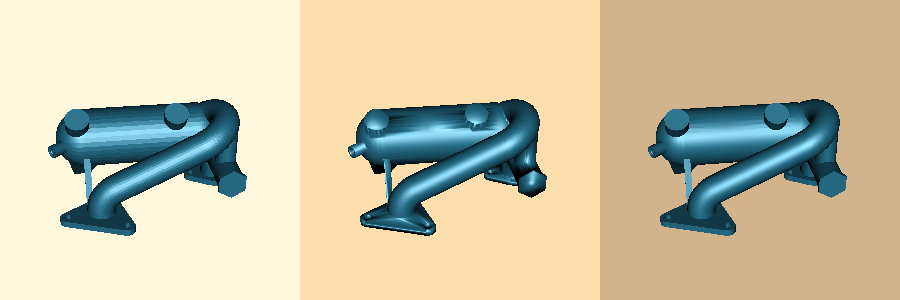
\includegraphics[width=0.96\linewidth]{Figure9-24a}
		\captionsetup{justification=centering}
		\caption{Original faceted model (left), Naive normal generation,(center), Split-edge normal generation(right) (\href{https://lorensen.github.io/VTKExamples/site/Cxx/Visualization/NormalsDemo/}{NormalsDemo.cxx} or \href{https://lorensen.github.io/VTKExamples/site/Python/Visualization/NormalsDemo/}{NormalsDemo.py})}
		\label{fig:Figure9-24a}
	\end{subfigure}
	\hfill
	\begin{subfigure}[h]{0.4\linewidth}
		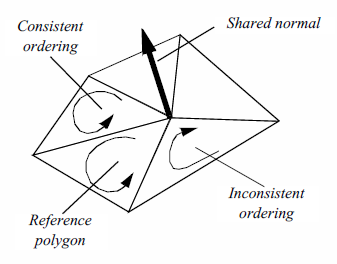
\includegraphics[width=0.96\linewidth]{Figure9-24b}
		\captionsetup{justification=centering}
		\caption{Normal computation}
		\label{fig:Figure9-24b}
	\end{subfigure}
	\caption{ Surface normal generation. Left -- faceted model without normals. Center -- sharp edges are poorly represented using shared normals as shown on the corners of this model. Right -- normal generation with sharp edges split.}\label{fig:Figure9-24}
\end{figure}

Gouraud and Phong shading (see \pageref{subsection:rasterization.phong}) can improve the appearance of rendered polygons. Both techniques require point normals. Unfortunately polygonal meshes do not always contain point normals, or data file formats may not support point normals. Examples include the marching cubes algorithm for general datasets (which typically will not generate surface normals) and the stereo lithography file format (does not support point normals). Figure \ref{fig:Figure9-24a}(left) shows a model defined from stereo-lithography format. The faceting of the model is clearly evident.

To address this situation we can compute surface normals from the polygonal mesh. A simple approach follows. First, polygon normals are computed around a common point. These normals are then averaged at the point, and the normal is renormalized (i.e., $\vert n \vert = 1$ ) and associated with the point. This approach works well under two conditions.

\begin{enumerate}

\item The orientation of all polygons surrounding the point are consistent as shown in Figure \ref{fig:Figure9-24b}. A polygon is oriented consistently if the order of defining polygon points is consistent with its edge neighbors. That is, if polygon $p$ is defined by points $(1,2,3)$, then the polygon edge neighbor $p_{23}$ must use the edge $(2,3)$ in the direction $(3,2)$. If not consistent, then the average point normal may be zero or not accurately represent the orientation of the surface. This is because the polygon normal is computed from a cross product of the edges formed by its defining points.

\item The angular difference in surface normals between adjacent polygons is small. Otherwise, sharp corners or edges will have a washed out appearance when rendered, resulting in an unsatisfactory image (Figure \ref{fig:Figure9-24a}(center)).

\end{enumerate}

To avoid these problems we adopt a more complex polygon normal generation algorithm. This approach includes steps to insure that polygons are oriented consistently, and an edge-splitting scheme that duplicates points across sharp edges.

To orient edges consistently we use a recursive neighbor traversal. An initial polygon is selected and marked ``consistent''. For each edge neighbor of the initial polygon, the ordering of the neighbor polygon points is checked --- if not consistent, the ordering is reversed. The neighbor polygon is then marked ``consistent''. This process repeats recursively for each edge neighbor until all neighbors are marked ``consistent''. In some cases there may be more than one connected surface, so that the process may have to be repeated until all polygons are visited.

\begin{figure}[htb]
    \centering
	\begin{subfigure}[h]{0.48\linewidth}
		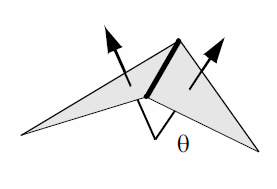
\includegraphics[width=0.96\linewidth]{Figure9-25a}
		\captionsetup{justification=centering}
		\caption{Feature edge)}
		\label{fig:Figure9-25a}
	\end{subfigure}
	\hfill
	\begin{subfigure}[h]{0.48\linewidth}
		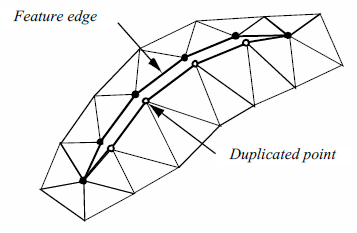
\includegraphics[width=0.96\linewidth]{Figure9-25b}
		\captionsetup{justification=centering}
		\caption{Exagerated splitting of feature edge}
		\label{fig:Figure9-25b}
	\end{subfigure}
	\caption{Computing feature angles (a) and splitting edges (b).}\label{fig:Figure9-25}
\end{figure}

A similar traversal method splits sharp edges. A sharp edge is an edge shared by two polygons whose normals vary by a user-specified feature angle. The feature angle between two polygons is the angle between their normals (Figure \ref{fig:Figure9-25a}). When sharp edges are encountered during the recursive traversal, the points along the edge are duplicated, effectively disconnecting the mesh along that edge (Figure \ref{fig:Figure9-25b}). Then, when shared polygon normals are computed later in the process, contributions to the average normal across sharp edges is prevented.

On some computers limitations on recursion depth may become a problem. Polygonal surfaces can consist of millions of polygons, resulting in large recursion depth. As a result, the depth of recursion can be specified by the user. If recursion depth exceeds the specified value, the recursion halts and the polygons on the boundary of the recursion become seeds to begin the process again.

Figure \ref{fig:Figure9-24a}(right) shows the result of the advanced normal generation technique with a feature angle of 60$^\circ$. Sharp edges are well defined and curved areas lack the faceting evident in the original model. The figure is shown with Gouraud shading.

\subsection{Decimation}

\begin{description}
	\item[Triangulation.] \label{subsec:decimation.triangulation} After deleting a point, the resulting hole must be retriangulated.
\end{description}

\subsection{Mesh Smoothing}
\label{subsec:mesh_smoothing}

\subsection{Visualizing Unstructured Points}
\label{subsec:visualizing_unstructured_points}

\subsection{Texture Algorithms}
\label{subsec:texture_algorithms}

\section{Putting It All Together}

\subsection{Connectivity}
\label{subsec:connectivity}

\section{Chapter Summary}

Dividing cubes is a scalar contouring operation that generates points rather than surface primitives such as lines or polygons. Dense point clouds appear solid because of the limited resolution of computer images.

Vector fields have a complex structure. This structure can be visualized using streamribbons, streamsurfaces, and streampolygons. The topology of a vector field can be characterized by connecting critical points with streamlines.

Tensor fields consist of three orthogonal vector fields. The vector fields are the major, medium, and minor eigenvectors of the tensor field. Hyperstreamlines can be used to visualize tensor fields.

Dataset topology operations generate triangle strips, extract connected surfaces, and compute surface normals. Decimation is a polygon reduction algorithm that reduces the number of triangles in a triangle mesh. Implicit modelling techniques can be used to construct swept surfaces and volumes. Unstructured points are easy to represent but difficult to visualize. Splatting, interpolation, and triangulation techniques are available to construct structure for unstructured points. Multivariate visualization is required for data of dimension four and higher. Data must be mapped to three dimensions before standard visualization techniques can be used. Parallel coordinates techniques are also available to visualize multivariate data.

Modelling algorithms extract geometric structure from data, reduce the complexity of the data or create geometry. Spatial extraction selects dataset structure and associated data attributes lying within a specified region in space. Subsampling reduces data by selecting every nth data point. A related technique, data masking, selects every nth cell. Subsets of a dataset can also be selected using thresholding, which selects cells or points that lie within a range of scalar values. Probing resamples data at a set of points. The probe produces a dataset that has the topology of the probe with data values from the probed dataset. Generating triangle strips can reduce storage requirements and improve rendering speeds on some systems. If a dataset has multiple disjoint structures, a connectivity algorithm can uniquely identify the separate structures. For polygonal data that does not have vertex normals defined, normal generation algorithms can compute these values that are suitable for interpolation by Gouraud or Phong shading. Decimation, another data reduction technique, removes triangles in ``flat'' regions and fills the resulting gaps with new triangles. Unstructured points present a challenge because the data does not have topology. Splatting represents each point in the data with a uniform sampling and accumulates these splats using implicit modelling techniques. Triangulation techniques build topology directly from the unstructured points.

Multidimensional visualization techniques focus on data that has many scalar data values for each point. Parallel coordinates is an interesting approach that plots the scalar values for a data point along a parallel axis. The observer looks for trends and relationships between the lines that represent each point's data.

Texture algorithms use texture coordinates and texture maps to select or highlight portions of a dataset. Texture thresholding assigns texture coordinates based on a scalar value. The scalar value and texture map determine how a cell or portion of a cell is rendered. Boolean textures extend this concept to 2D and 3D. Careful design of a boolean texture map permits the ``clipping'' of geometry with combinations of implicit surfaces. Texture can also be used to animate vector fields.

\section{ Bibliographic Notes}

Dividing cubes is an interesting algorithm because of the possibilities it suggests \cite{Cline88}. Point primitives are extremely simple to render and manipulate. This simplicity can be used to advantage to build accelerated graphics boards, perform 3D editing, or build parallel visualization algorithms.

Many plotting and visualization systems use carpet plots extensively. Carpet plots are relatively easy to represent and render. Often 2D plotting techniques are used (i.e., lighting and perspective effects ignored). Check \cite{Wang90} for additional information on rendering carpet plots.

In recent years a number of powerful vector visualization techniques have emerged. These techniques include streamsurfaces \cite{Hultquist92}, streampolygons \cite{Schroeder91}, vector field topology \cite{Helman91} \cite{Globus91}, streamballs \cite{Brill94}, and vorticity visualization \cite{Banks94}. The streamballs technique is a recent technique that combines techniques from implicit modeling. You may also wish to see references \cite{Crawfis92} \cite{vanWijk93} and \cite{Max94}. These describe volume rendering and other advanced techniques for vector visualization, topics not well covered in this text.

Some abstract yet beautiful visualization images are due to Delmarcelle and Hesselink \cite{Delmarcelle93}. Their rendering of hyperstreamlines reflect the underlying beauty and complexity of tensor fields.

Polygon reduction is a relatively new field of study. SIGGRAPH '92 marked a flurry of interest with the publication of two papers on this topic \cite{Schroeder92a} \cite{Turk92}. Since then a number of valuable techniques have been published. One of the best techniques, in terms of quality of results, is given by \cite{Hoppe93}, although it is limited in time and space because it is based on formal optimization techniques. Other interesting methods include \cite{Hinker93} and \cite{Rossignac93}. A promising area of research is multiresolution analysis, where wavelet decomposition is used to build multiple levels of detail in a model \cite{Eck95}. The most recent work in this field stresses progressive transmission of 3D triangle meshes \cite{Hoppe96}, improved error measures \cite{Garland97}, and algorithms that modify mesh topology \cite{Popovic97} \cite{Schroeder97}. Most recently an extensive book on the technology is available including specialized methods for terrain simplification \cite{Luebke02}.

Triangle strip generation is an effective technique for achieving dramatic improvements in rendering speed and reductions in data handling. The reference by \cite{Evans96} describes other triangle strip generation algorithms as well as presenting some of the most effective techniques to date.

The use of texture for visualization is relatively unexploited. This has been due in part to lack of texture support in most graphics software and hardware. This is now changing, as more vendors support texture and software systems (such as OpenGL) that provide an API for texture. Important references here include the boolean textures \cite{Lorensen93} and surface convolution techniques \cite{Cabral93} \cite{Stalling95}.

Unstructured or unorganized point visualization is likely to play a prominent role in visualization as the field matures and more complex data is encountered. Nielson et al. have presented important work in this field \cite{Nielson91a}.

Multidimensional visualization is another important focus of visualization research \cite{Bergeron89} \cite{Mihalisin90}. Much real-world data is both unstructured and multidimensional. This includes financial databases, marketing statistics, and multidimensional optimization. Addressing this type of data is important to achieve future advances in understanding and application. Feiner \cite{Feiner90} has presented a simple projection method combined with virtual reality techniques. \cite{Inselberg87} has introduced parallel coordinates. These techniques have been shown to be powerful for many types of visual analysis.

\printbibliography

\section{Exercises}

\begin{enumerate}

\item Describe an approach to adapt dividing cubes to other 3D cell types. Can your method be adapted to 1D and 2D cells?

\item Discuss the advantages and disadvantages of representing surfaces with points versus polygons.

\item Streamribbons can be constructed by either i) connecting two adjacent streamlines with a surface, or ii) placing a ribbon on the streamline and orienting the surface according to streamwise vorticity vector. Discuss the differences in the resulting visualization.

\item Write the following programs to visualize velocity flow in the combustor.

    \begin{enumerate}

    \item Use vtkProbeFilter and vtkHedgeHog.

    \item Use vtkProbeFilter and vtkStreamLine.

    \item Use vtkProbeFilter and vtkWarpVector.

    \item Use vtkProbeFilter and vtkVectorNorm.

    \item Use vtkProbeFilter and vtkVectorDot.

    \end{enumerate}

\item Describe a method to extract geometry using an arbitrary dataset. (That is, extract geometry that lies within the culling dataset.) (Hint: how would you evaluate in/out of points?)

\item The filter vtkPolyDataNormals is often used in combination with the filters vtkSmoothPolyData and vtkContourFilter to generate smooth isosurfaces.

    \begin{enumerate}

    \item Write a class to combine these three filters into one filter. Can you eliminate intermediate storage?

    \item How much error does vtkSmoothPolyData introduce into the isosurface? Can you think of a way to limit the error?

    \item What is the difference between the surface normals created by vtkMarchingCubes and vtkPolyDataNormals?

    \end{enumerate}

\item Assume that we have a database consisting of interest rate R, monthly payment P, monthly income I, and days payment is late L.

    \begin{enumerate}

    \item If R, P, I are all sampled regularly, how would you visualize this data?

    \item If all data is irregularly sampled, list three methods to visualize it.

    \end{enumerate}

\item Why do you think triangle strips are often faster to render than general polygons?

\item The normal generation technique described in this chapter creates consistently oriented surface normals.

    \begin{enumerate}

    \item Do the normals point inside or outside of a closed surface?

    \item Describe a technique to orient normals so that they point out of a closed surface.

    \item Can surface normals be used to eliminate visible triangles prior to rendering? (Hint: what is the relationship between camera view and surface normal?)

    \end{enumerate}

\item Describe a technique to partially threshold a cell (i.e., to cut a cell as necessary to satisfy threshold criterion). Can an approach similar to marching cubes be used?

\item The class vtkRendererSource allows us to use the rendered image as a texture map (or image data dataset). Write a program to construct iterated textures, that is textures that consist of repeated images. Can the same image be generated using texture coordinates?

\item Describe how you would modify the decimation algorithm to treat general polygons.

\item Several examples in the text (e.g., deciFran.tcl and deciHawa.tcl) use the class vtkDecimate. Modify these examples to use the topology modifying progressive decimation algorithm (implemented in vtkDecimatePro). How much greater reduction can you achieve?


\end{enumerate}